\chapter{Implementation}

 \section{Rendering}  
    Rendering code is split into two parts, in different places. There is a rendering "component" in the components/render folder.
    This component exports basic rendering functions for loading and drawing sprites etc, but does not deal with the rendering loop, it has a draw() function which will swap the buffers, and must be called manually.   
    It is essentially a wrapper for a low level rendering library, with some application specific logic (it has the ability to draw "levels", ie Level::Level objects representing an isometric level of the game, and also load the proprietary CEL and CL2 formats).
    This code is placed in a component because it is common to both the freeablo game engine and the image viewer.
    
    The rendering component can be backed by either SDL1 or 2, and this can be set at compile time using the USE\_SDL2 cmake variable. SDL2 provides better support for hardware acceleration, and as a result, normally produces much higher framerates. SDL1 was retained as most linux distributions don't ship SDL2 yet, and also some older platforms are no longer supported in SDL2.
    
    \mbox{}
    
    The second part is the code that controls the actual rendering for the game. This is located in apps/freeablo/farender. Essentially, this contains a class FARender::Renderer, that manages sprite loading and render looping for the game engine.
    
    \begin{center}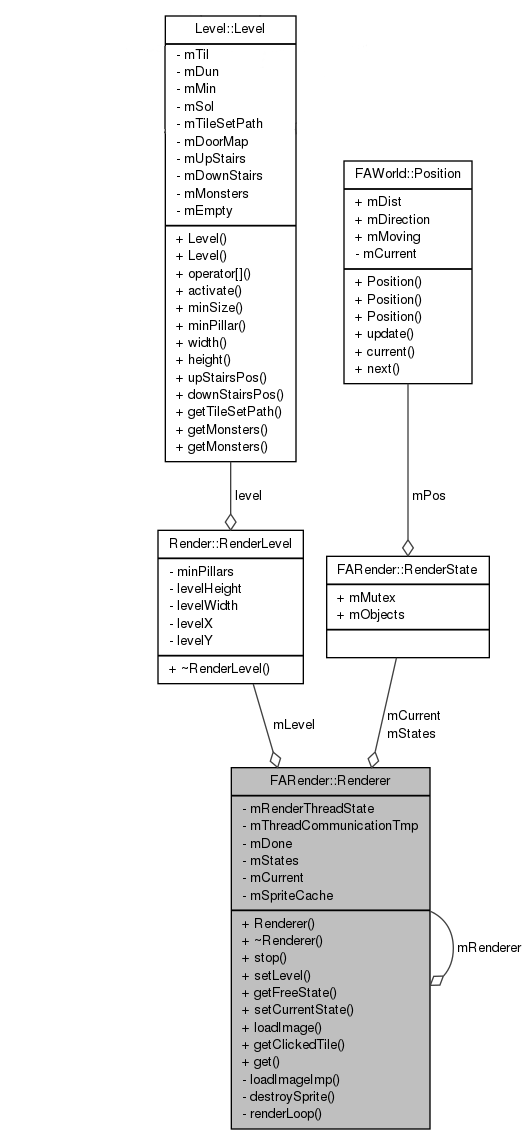
\includegraphics[scale=0.4]{renderer}\end{center}
      
    When created, the Renderer class starts up a separate thread, which then loops until the object is destroyed. Each iteration, the renderer will draw the level, and a list of objects, which are essentially just sprites and locations.
    The game engine communicates with the renderer through a triple buffered system.
    
    \subsection{Triple Buffering}
    The Renderer creates three RenderState objects, each of which is just a container for a number of sprites and their corresponding locations, and a location on which to centre the camera.
    Each iteration of the game loop, after processing the game logic for the current tick, the engine will "fill" a render state, and pass it off to the renderer. This filling is basically just a flattening of game state, removing all information about objects other than sprite and location, and dumping it into the state.
    Three states are used, as at any given point the renderer can be drawing a state, and the game loop can be filling one, so with three we are always guaranteed to have one free.
    Locks are used when rendering and filling a state to ensure that we are never reading and writing the same state at the same time.
    As the game and render loops can (and probably are) iterating at different rates, when the render loop is going faster, some render states will never be drawn to screen, but this is acceptable, as whatever is on screen at any given moment is an accurate portrayal of game state to the granularity allowed by the iteration speed of the renderer, which is determined by the speed of the processor and GPU (no framelimit is set on the renderer).
    
    \subsection{Threading Issues}
    It is a requirement of the library that all SDL calls occur in the main thread, so there are some synchronisation issues with various actions such as loading sprites and changing level. The restriction that it be the main thread is the reason that rendering takes place in the main thread, with the game loop occurring in a separate one, which at first seems counterintuitive.
    Each action that must take place in the render thread, but is called from the game thread is given an entry in the RenderThreadState enum. The Renderer class has a member, mRenderThreadState, which is an atomic instance of the RenderThreadState enum type (atomicity achieved using boost::atomic). On each iteration of the render loop, the value of this synchronisation variable is checked. When it is set to running, the game can render the frame, otherwise, it executes the action corresponding to the current value, then resets itself to allow the render to continue, and the caller to know that it has completed execution. Passing values between threads is done via a void* member called mThreadCommunticationTmp.
    
    For example, when loading a sprite, the loadImage function (which is called from the game thread) will save the image path into the void* then set mRenderThreadState to loadSprite, and enter a busy wait for mRenderThreadState == 0.
    When the render thread encounters mRenderThreadState == loadSprite, it will create a new Sprite object on the heap. It will then pull the path out from  the void*, then call loadImageImp with that as the parameter (the function that implements the actual image loading), saving the result into the heap variable it just created.
    When that function returns, it will assign mThreadCommunticationTmp the pointer to the new heap Sprite, and set mRenderThreadState back to running.
    The game thread will now see that it has completed, and return the sprite as required.
        
    \section{Input}
    
    \begin{center}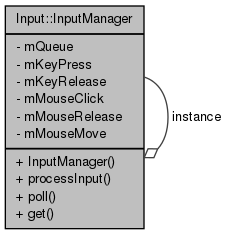
\includegraphics[scale=0.5]{inputmanager}\end{center}
    Input is handled in the game loop thread, with the Input::InputManager singleton class. Like rendering, it is done using SDL, so it is also abstracted away in the Input component.
    The input component consists of an object to which one binds callbacks. These callbacks are then executed when the processInput() method is called, if the corresponding input actions have occurred.
  	
  	Unfortunately, while the input is used in the game loop thread, the specifics of SDL require that the SDL event polling occur on the main thread. As such, the raw input polling is done inside the render loop, by calling poll(). 
  	For each SDL event generated in the render loop, an event is added onto a concurrent queue. The events on this queue are contained in a structure that very much resembles the parts of the SDL\_Event union that we actually use.
  	The game loop then calls processInput, which pops events off the queue, and it is here that the callbacks are executed.

\section{Game Loop}
	As explained above, the game loop occurs in a secondary thread. The game loop is essentially a huge while loop  located (for now) in the realmain function in the main.cpp file in apps/freeablo.
	It executes at a fixed rate of 120 time per second, and is responsible for applying user inputs and advancing game state. The fixed execution rate is required for the engine to be deterministic.
	
	Game state is stored in the FAWorld::World object. This object is essentially a container for all object in the world. A call to World::update() will update the positions and animations of these objects.
	The World class is also responsible for filling RenderState objects, via the fillRenderState method.
	
\section{Diablo.exe}
	Unfortunately, some of the information required for the game is hardcoded into the original executable.
	The exact extent to which this issue will occur has not yet been fully determined, but so far the freeablo engine is extracting monster and npc data.
	
	To deal with this problem, the DiabloExe component was created. In order for this to be version independent, the DiabloExe class uses a number of ini files to specify data locations. First the file is hashed to determine which version we are using, then the corresponding ini file is loaded according to that hash. These ini files contain the addresses of the relevant data within the file, which can then be loaded.
	
	By abstracting this process out into a generic loader class, we avoid having all sorts of nasty hex addresses cluttering up the source files where the information is actually needed.
	
	Of course, in order to load this information, one first needs to know where it is, which can be a nontrivial task in itself. Fortunately, there has been extensive reverse engineering work done on diablo in the past. Much of the information needed has addresses documented on the website for The Dark Mod\cite{dmodhex}. Currently, freeablo only has an ini file for version 1.09 of Diablo, as that is the version documented in the above location (this is the second most recent patch for Diablo).
	
	However, not all the necessary information is documented there, for example the locations of the NPCs in the town had to be figured out unassisted. For this, the Hex Rays IDA\cite{hexrays} decompiler proved fantastically useful.

\section{FAIO}
	The FAIO component is responsible for file IO in freeablo (or, more accurately, just input, as it does not allow file writing).
	The game data files for Diablo are all stored in the DIABDAT.MPQ file. MPQ is a proprietary archive format originally developed by Blizzard for Diablo, and used in all their games since.
	
	Thankfully, a library exists for using these archives, named StormLib\cite{stormlib}. It provides an fopen / fread etc style api for mpq files.
	FAIO is essentially a wrapper around this library, that allows the user to override files by placing them on the local filesystem. This means that when requested to open a file, it will search for the file in the local filesystem, and if it finds it there, use that, otherwise look in the MPQ file.
	This behaviour is based on that of the BSA files in the Elder Scrolls game series.
	
\newpage
	
\section{Level Generation}
    Level generation in freeablo is performed in a number of stages. The first stage is the creation of a flat map. This is the part with interesting algorithms.
    After that, the map is turned isometric, and then has monsters place + random variance introduced into the tileset, but neither of these merit discussion.

    \mbox{}

    The level generation algorithm used in freeablo is borrowed from a game called TinyKeep\cite{tinykeep}, the author of which has published the algorithm he developed\cite{tinygen}.
    The algorithm is designed to create rooms connected by corridors on a grid.
    There are a number of steps which are executed in sequence to produce this map.
    \begin{itemize}
        \item
        {
            The first step is to place a number of rooms in the centre of the grid, keeping them within a small circle placed there.
            The rooms can overlap within this circle, and indeed are expected to. The number of rooms, and the radius of the circle in which they are placed
            should be related in some way to the size of the map being generated. The width, height, and position within the circle of the rooms is randomly generated, with the randomness for width and height biased so we receive more small rooms than large ones.    
        }
        \item
        {
            After this, we use separation steering to move the rooms away from each other until none of them overlap.
        }
        \item
        {
            At this point, we split the rooms into two groups, by thresholding on size. Those over the threshold value (area of 30 was used in the freeablo engine) are said to be real rooms, and the rest are said to be corridor rooms. The bias when generating levels mentioned above ensures that most rooms are chosen to be corridor rooms.
        }
        \item
        {
            We construct a graph of real rooms, where each room is connected to each other room. We then calculate the minimum spanning tree of this graph. Now we know that if we apply corridors corresponding to the edges on this graph, each room will be accessible from each other one.
        }
        \item
        {
            Because the graph we constructed above is a tree, there will be no cycles, however a small number of cycles is desirable in a dungeon crawler, so we add in a number of random edges to create some.
        }
        \item
        {
            For every edge on the graph, we create an L-shaped corridor on the map, joining the two rooms that correspond to that edges vertices.
            This is where the corridor rooms come into effect. For each corridor room that the corridors intersect, we add the shape of that room onto the corridor. In this way, we end up with lumpy corridors that can resemble large rooms themselves, and do not just look like simple L shapes.
        }
    \end{itemize}
    
    Example levels generated:\\ 
    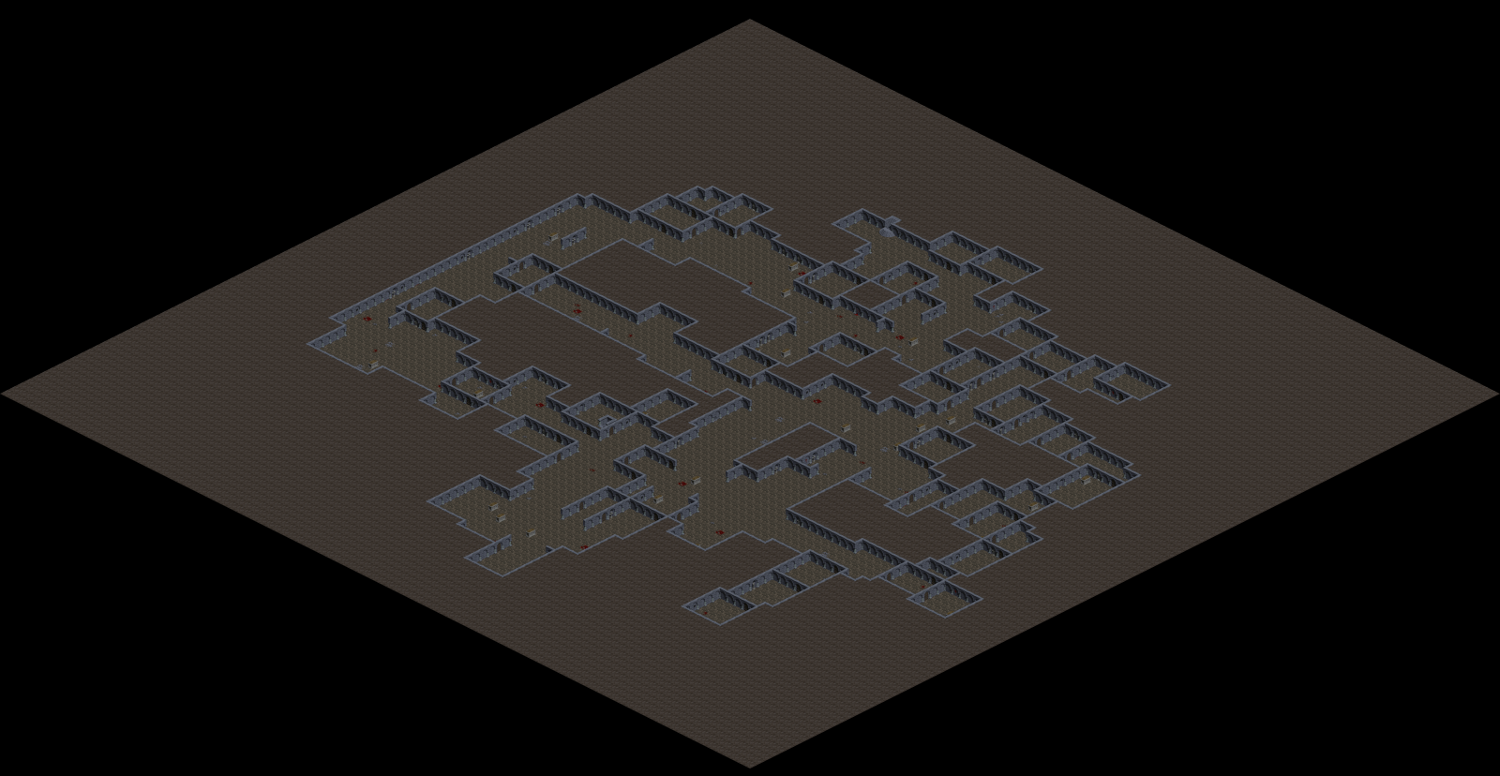
\includegraphics[scale=0.2]{rnd1}\\   
    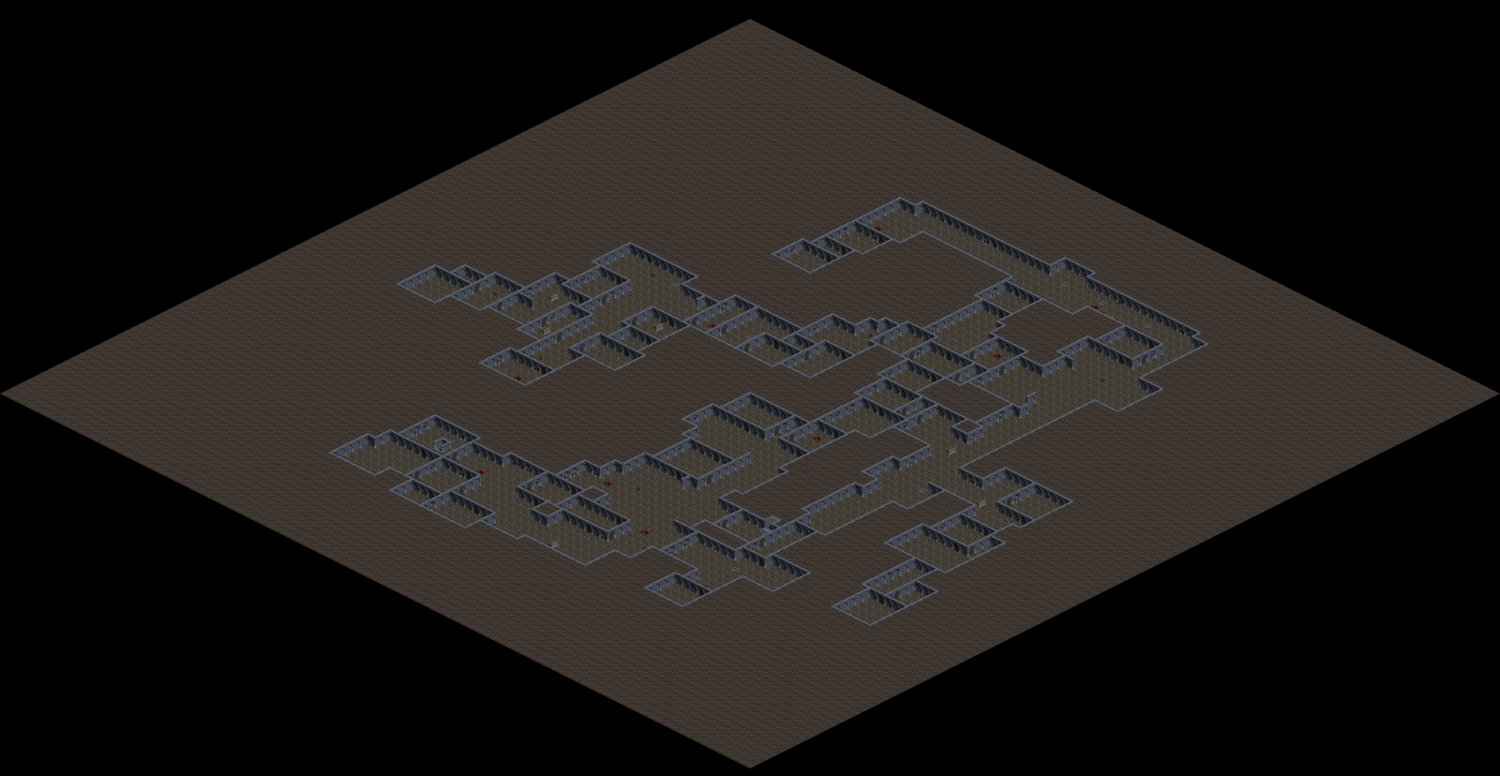
\includegraphics[scale=0.2]{rnd2}\\
    
   	\newpage
    
   	\section{Libraries}
       	\subsection{2d graphics libraries}
    	There seems to be 3 different options for 2d graphics in C++:
    	\begin{itemize}
    	    \item{SDL}
    	    \item{Allegro}
    	    \item{SFML}
    	\end{itemize}
    	
    	Of the above, all are written in plain C, except Allegro, which is C++.
    	I have decided to use SDL for this project, as I am already familiar with it.
    	As described above, both SDL 1 and 2 were used, with the version being configurable at compile time through a cmake varaible.
    	
    	\subsection{Cross Platform}
        The Boost C++ library addresses many of the problems with writing portable C++ code today.
     	Heavy use has been made of various parts of boost, mostly boost::thread and boost::filesystem.
        
        \subsection{Audio}
        SDL has a module for audio, SDL\_sound\cite{sdls}, but it has not been updated since 2008.
        FFMPEG's library, libavcodec\cite{libavcodec} supports a large number of formats.
        OpenAL seems to be popular also, but is no longer FOSS.
        Audio has not yet been implemented, but when it is I would lean towards FFMPEG, as it can also be used to decode the intro videos.
        
        \subsection{StormLib}
        StormLib\cite{stormlib} is a library for accessing files in Blizzard MPQ format archives.
        It was chosen because it is the only viable option. Others do exist, but are no longer maintained.
